\begin{figure}
\begin{tabular}{cc}
\begin{subfigure}[b]{0.55\textwidth}
\begin{center}
\begin{allLangEnvFoot}
~{\tiny \textcolor{mygray}{S0:}}~ OptStr strchr (Str s, i8 c) {
~{\tiny \textcolor{mygray}{S1:}}~   while ${\tt true}$:
~{\tiny \textcolor{mygray}{S2:}}~     assume ${\tt \neg (s\ is\ SInvalid)}$;
~{\tiny \textcolor{mygray}{S3:}}~     if s is SNil:
~{\tiny \textcolor{mygray}{S4:}}~       if c == ${\tt 0_{i8}}$: return Found(s);
~{\tiny \textcolor{mygray}{S5:}}~       return NotFound();
~{\tiny \textcolor{mygray}{S6:}}~     i8 ch $\coloneq$ s.char; // (s is SCons)
~{\tiny \textcolor{mygray}{S7:}}~     if c == ch: return Found(s);
~{\tiny \textcolor{mygray}{S8:}}~     s $\coloneq$ s.tail;
~{\tiny \textcolor{mygray}{SE:}}~ }
\end{allLangEnvFoot}
\end{center}
\caption{\label{fig:llStrchrSpecIR}Strchr Spec IR Program}
\end{subfigure}%
&
\begin{subfigure}[b]{0.46\textwidth}
\begin{center}
\begin{allLangEnvFoot}
~{\tiny \textcolor{mygray}{\ \ \ }}~ char* strchr(char* t, int c);
~{\tiny \textcolor{mygray}{}}~
~{\tiny \textcolor{mygray}{C0:}}~ i32 strchr (i32 t, i32 c) {
~{\tiny \textcolor{mygray}{C1:}}~   i8 ch $\coloneq$ ${\tt bvextract_{7:0}(c)}$
~{\tiny \textcolor{mygray}{C2:}}~   while $\mathrm{\tt t[0_{i32}]^m_{i8} \neq ch}$:
~{\tiny \textcolor{mygray}{C3:}}~     if $\mathrm{\tt t[0_{i32}]^m_{i8} == 0_{i8}}$:
~{\tiny \textcolor{mygray}{C4:}}~       return ${\tt 0_{i32}}$;
~{\tiny \textcolor{mygray}{C5:}}~     t $\coloneq$ t + ${\tt 1_{i32}}$
~{\tiny \textcolor{mygray}{C6:}}~   return t;
~{\tiny \textcolor{mygray}{CE:}}~ }
\end{allLangEnvFoot}
\end{center}
\caption{\label{fig:llStrchrCArrIR}Generic Strchr C IR Program using Array}
\end{subfigure}%
\\
\begin{subfigure}[b]{0.55\textwidth}
\begin{center}
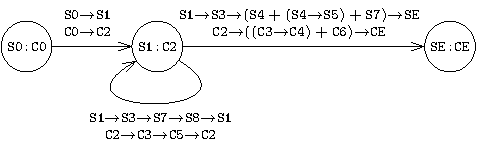
\includegraphics[scale=0.87]{chapters/figures/figStrchrProductCfg.pdf}
\end{center}
\caption{\label{fig:llStrchrProduct}XXX}
\end{subfigure}%
&
\begin{subfigure}[b]{0.50\textwidth}
\begin{center}
\begin{footnotesize}
\begin{tabular}{|c|l|}
\hline
\tt PC-Pair & \multicolumn{1}{c|} {\tt Invariants} \\
\hline
\hline
${\tt (S0:C0)}$ &
${\tt {\scriptsize \circled{P1}}\  s_{S}\indEq{}Cstr^{char[]}_{m}(t_{C})}$ \\ & ${\tt {\scriptsize \circled{P2}}\ c_{S}=bvextract_{7:0}(c_{C})}$ \\
\hline
${\tt (S1:C2)}$ &
${\tt {\scriptsize \circled{I1}}\  s_{S}\indEq{}Cstr^{char[]}_{m}(t_{C})}$ \\ & ${\tt {\scriptsize \circled{I2}}\  c_{S}=ch_{C}}$ \\
\hline
${\tt (SE:CE)}$ &
${\tt {\circled{E}}\  ret_{S}\indEq{}Cstr^{char[]}_{m}(ret_{C})}$ \\
\hline
\end{tabular}
\end{footnotesize}
\end{center}
\caption{\label{fig:llStrchrInvTable}XXX}
\end{subfigure}%
\\
\end{tabular}
\caption{\label{fig:llStrchr}XXX}
\end{figure}